% Это основная команда, с которой начинается любой \LaTeX-файл. Она отвечает за тип документа, с которым связаны основные правил оформления текста.
\documentclass{article}

% Здесь идет преамбула документа, тут пишутся команды, которые настраивают LaTeX окружение, подключаете внешние пакеты, определяете свои команды и окружения. В данном случае я это делаю в отдельных файлах, а тут подключаю эти файлы.

% Здесь я подключаю разные стилевые пакеты. Например возможности набирать особые символы или возможность компилировать русский текст. Подробное описание внутри.
\usepackage{packages}

% Здесь я определяю разные окружения, например, теоремы, определения, замечания и так далее. У этих окружений разные стили оформления, кроме того, эти окружения могут быть нумерованными или нет. Все подробно объяснено внутри.
\usepackage{environments}

% Здесь я определяю разные команды, которых нет в LaTeX, но мне нужны, например, команда \tr для обозначения следа матрицы. Или я переопределяю LaTeX команды, которые работают не так, как мне хотелось бы. Типичный пример мнимая и вещественная часть комплексного числа \Im, \Re. В оригинале они выглядят не так, как мы привыкли. Кроме того, \Im еще используется и для обозначения образа линейного отображения. Подробнее описано внутри.
\usepackage{commands}

% Пакет для титульника проекта
\usepackage{titlepage}

% Пакет для кода
\usepackage{listings}

% Здесь задаем параметры титульной страницы
\setUDK{004.942}
% Выбрать одно из двух
% \setToResearch
\setToProgram

\setTitle{Торговая система для крипто-бирж}

% Выбрать одно из трех:
% КТ1 -- \setStageOne
% КТ2 -- \setStageTwo
% Финальная версия -- \setStageFinal
% \setStageOne
\setStageTwo
%\setStageFinal

\setGroup{209}
%сюда можно воткнуть картинку подписи
\setStudentSgn{}

\setStudentDate{17.02.2022}
\setAdvisor{Казаков Евгений Александрович}
\setAdvisorTitle{разработчик}
\setAdvisorAffiliation{Facebook inc.}
\setAdvisorDate{17.02}
\setGrade{10}
%сюда можно воткнуть картинку подписи
\setAdvisorSgn{}
\setYear{2022}


% С этого момента начинается текст документа
\begin{document}

% Эта команда создает титульную страницу
\makeTitlePage

% Данное окружение оформляет аннотацию: краткое описание текста выделенным абзацем после заголовка
\begin{abstract}
Говорить о крипте можно много, но интереснее знать, как она устроена изнутри и как на ней можно заработать. Эти цели мы поставили в своей работе.


Результатами стали:

\begin{enumerate}

\item Коннекторы для подключения к биржам, чтобы было просто с ними взамодействовать через API.

\item Маркет-мейкинг стратегия.

\item Модель на основе решающих деревьев и градиентного бустинга, предсказывающая направление рынка, базирующаяся на информации об индикаторах.

\item Арбитражная стратегия, которая торгует исходя из курса на другой бирже.

\end{enumerate}


Пайплан нашей работы был такой:

\begin{enumerate}
\item Сначала мы искали торговые стратегии. Рассматривали как самые современные, так и достаточно старые, которые можно переосмыслить с современными технологиями.
\item Потом мы собирали данные для экспериментов. Для этого написали функцию в коннекторе, куда можно подать интересующий интервал времени, и она выдаст датасет с историческими данными.
\item Далее мы очищали данные от мусора, чтобы эксперимент сделать как можно точнее
\item И на самом интересном шаге -- эксперименте -- мы прототипировали стратегию в юпитер-ноутбуке и прогоняли на исторических данных, чтобы понять, можно ли что-то заработать или нет.
\item На последнем шаге мы переписывли нашу стратегию из юпитер-ноутбуков в питоновские файлы, оптимизировали стратегию, чтобы она работало как можно быстрее и занимала как можно меньше памяти. Нам было важно писать код так, чтобы его можно было переиспользовать в других стратегиях, и не делать одну и ту же работу несколько раз.
\end{enumerate}


\end{abstract}

% Здесь будет автоматически генерироваться содержание документа
\tableofcontents

\section{Введение}

\subsection{Актуальность проблемы}
Все говорят о криптовалютах, но толком никто ничего о них не знает. Мы решили разобраться, как устроен блокчейн и технологии вокруг него, какие есть проблемы и как с ними справляются.

Одна из проблем больших блокчейнов, таких как Bitcoin и Ethereum, -- высокая загруженность. Они критически не справляются с нагрузкой. Из-за того, что сеть Эфириума может обрабатывать лишь 15 транзакций в секунду, комиссия, которую нужно заплатить, чтобы транзакция была одной из этих 15, доходит до \$100, что делает любой токен на блокчейне непригодным для использования в качестве обменной валюты.


Чтобы снизить нагрузку на мэйннет\footnote{Основная сеть блокчейна, на которой криптовалюта имеет реальную стоимость. Есть также сети для тестирования разработок. На них валюту можно получить по запросу от специальных адресов}, были разработаны и все еще разрабатываются несколько альтернативных решений, которые одним словом называются \texttt{Layer-2} решения. Это надстройки над блокчейном, которые увеличивают пропускную способность и скорость в ущерб децентрализованности.


Мы считаем, что пока не придумали более изящного способа достичь тех же результатов, которые дают L2 решения, данная технология будет развиваться, а актуальности нашей темы будет расти.


\subsection{Цели и задачи}
\subsubsection{Цель}
Написать трейдинг систему, которая сможет стабильно выходить в плюс.
\subsubsection{Задачи}
\begin{itemize}
\item Проведение исследований по стратегиям трэйдинга.
\item Проверка работоспособность стратегий.
\item Создание инфраструктуры, позволяющей взаимодействовать с биржей автоматизированно.
\item Сбор данных и обучение модели.
\item Написание программы, совершающей сделки.
\item Обзор и сравнительный анализ источников и аналогов
\end{itemize}
К сожалению, выбранная нами тема мало освещается в источниках любого вида: никто не захочет делиться прибыльной стратегией. Многое нам приходилось и придется делать с нуля.
\subsection{Статьи}
Тем не менее, существуют статьи, описывающие некоторые возможные подходы к написанию алгоритмов HFT. Например, есть ресурс~\cite{HftBattle}, на котором описывается стратегия маркет-мейкинга, аналог которой мы попытались реализовать. Но материалы такого рода, находящиеся в открытом доступе, с течением времени теряют свою актуальность: если большое количество участников рынка придерживается одной схемы действий, то вскоре она перестает приносить прибыль. По этой причине мы старались не ориентироваться на подобные источники.
\subsection{Документация бирж}
Основным же источником информации для нас служила документация API~\cite{DydxDocs}~\cite{BinanceDocs} бирж, к которым мы подключались. С помощью нее был написан коннектор, инкапсулирующий процесс подключения и взаимодействия с биржей, произведен сбор необходимой информации: список сделок за последний месяц, состояние о счете и т.п.
\subsection{Документация библиотек}
Для машинного обучения мы использовали CatBoost~\cite{CatboostDocs} — это библиотека от Яндекса для градиентного бустинга, надстройки над решающими деревьями. КэтБуст для нас лучшее решение, потому что это самая быстрая библиотека для классификации среди аналогов и проста в использовании.

\subsection{Аналоги}
На крипто валютном рынке существует множество торговых ботов, но информации об их характеристиках и принципах работы практически нет. Мы можем судить об их доходности, лишь по каким-то сомнительным заявлениям или косвенным признакам. В открытом доступе в основном находятся боты, которые предоставляют лишь интерфейс взаимодействия с биржей ~\cite{CryptoTradingBot}~\cite{FreqTrade}: “ручная” покупка и продажа токенов, выставление лимитных ордеров и т.п.. Такие решения не представляют для нас никакого интереса.

Так достойных аналогов в свободном доступе нет, функциональные и нефункциональные требования нам пришлось придумывать самим. К счастью, они достаточно интуитивны.

\subsection{Описание функциональных требований к программному проекту}

\subsubsection{Коннектор к бирже}

В программе должны быть коннекторы к биржам. Это класс, в конструктор которого подаются приватные ключи кошельков. После этого можно работать с биржей: смотреть информацию о счете, валютаю, отправлять и отменять ордера. Надо реализовать функционал, который предоставляет апи, чтобы можно было его использовать в трейдинг-стратегиях.

Примеры использования функций класса, который способен взаимодействовать с биржами по API:

\begin{itemize}

\item Отправка ордеров
\begin{verbatim}
connector.send_order(
        symbol=ETH_USD, side=BUY, price=1, quantity=0.1
)
\end{verbatim}

\item Получение текущих позиций
\begin{verbatim}
connector.get_our_positions(
        opened=True, symbol=ETH_USD
)
\end{verbatim}

\item Информация о конкретном рынке
\begin{verbatim}
connector.get_symbol_info(market=ETH_USD)
\end{verbatim}

\end{itemize}

\subsubsection{Сбор данных}
Нужно обеспечить удобный механизм сбора исторических данных с бирж, на которых будет тестироваться и обучаться система. Удобно реализовать такие функции в коннекторе, ведь у него уже есть соединение с биржей.

Пример функции для сбора данных:
\begin{itemize}
\item Получение трейдов за определенный промежуток времени
\begin{verbatim}
connector.get_historical_trades(
        market=BTC_USD,
        begin="2021-12-12 09:00:00",
        end="2021-12-12 12:00:00"
)
\end{verbatim}
\end{itemize}

Также в коннекторе может быть функционал, позволяющий собирать данные в прямом эфире и сохранять их в архив, если эти исторические данные не предоставляет биржа.

\subsubsection{Измерение скорости соединения}
Так как счет идет на миллисекунды, мы всегда должны иметь четкое представления, какое время у нас займет отправка и получения пакета данных. Для этого должен быть предусмотрен отдельный модуль, который будет замерять скорость соединения с различными сервисами. Он тоже основывается на коннекторе, так как он уже умеет соединяться с биржей.

Примеры использования функций класса для измерения скорости коннектора:
\begin{itemize}
\item Измерение скорости
\begin{verbatim}
speed_measure = SpeedMeasure(connector)
speed_measure.get_connector_funcs_exec_times(
        market=ETH_USD,
        side=BUY,
        iters_num=10,
        filename="connector_funcs_exec_times.json",
    )
\end{verbatim}

\item Измерение задержки до биржи
\begin{verbatim}
speed_measure.get_orders_processing_delays(
        market=ETH_USD,
        side=BUY,
        orders_num=10,
        filename="orders_processing_delays.json",
)
\end{verbatim}
\end{itemize}

\subsubsection{Машинное обучение}
Индикаторов, по которым можно строить прогнозы, очень много, поэтому ручными методами не получится подобрать правильное соотношение весов. Здесь нужно машинное обучение, которое принимает на вход пред обработанные данные сделок, а на выход выдает модель, которую можно использовать в трейдинг-стратегии. Важно, чтобы модель была устойчива к тому, что в датасет добавляется или убирается индикаторы.
Примеры использования

\subsection{Описание нефункциональных требований к программному проекту}

\subsubsection{Безопасность}
Финансы — чувствительная тема, поэтому наша программа не должна допускать утечек данных о кошельках и приватных ключах. Нужно обеспечить безопасное хранение.

\subsubsection{Отказоустойчивость}
Во время трейдинга торговая система получает сотни обновлений от разных бирж, их обрабатывает, строит прогнозы и торгует. Нужно сделать так, чтобы система была готова к большим нагрузкам, и поведение было однозначно определено. Еще нужно проработать быстрое отключение торговой системы от торгов, если ее поведение станет неадекватным, и можно было бы быстро закрыть открытые заявки.

\subsubsection{Скорость}
В трейдинге важна каждая миллисекунда, поэтому цель — минимизировать время обработки, отправки и принятия данных.

\subsubsection{Переиспользование кода}
Нужно выстроить архитектуру проекта так, чтобы можно было быстро и легко тестировать свои гипотезы, поэтому код, который есть в проекте, должен быть написан так, чтобы его можно было легко понять и переиспользовать в других местах.

\subsubsection{Масштабируемость}
Система должна быть расширяема на несколько бирж и потенциально работать с большим количеством предсказательных моделей.

\section{Коннекторы}

Чтобы программа могла торговать, ей нужно подключиться к биржей. У выбранных нами бирж есть python-клиенты (python-binance и dydx-v3-python), позволяющие реализовать соединение. Итак, в нашем проекте есть 2 класса-коннектора, BinanceConnector и DydxConnector, с достаточно похожим функционалом.

\subsection{BinanceConnector}

\href{https://github.com/dexety/dex-trading-system/blob/main/connectors/binance/connector.py}{\texttt{BinanceConnector}}

\begin{definition}
Инструмент -- пара торгующихся на бирже валют
\end{definition}
\begin{definition}
Стакан -- таблица лимитных заявок на покупку и на продажу
\end{definition}

В конструкторе коннектор получает полученные из личного кабинета binance публичный и приватный ключи API для идентификации пользователя и список интересующих инструмент. Библиотека python-binance предоставляет класс синхронного клиента, Client. Методы этого класса используются в следующих функциях коннектора:

\begin{itemize}
    \item \texttt{get\_all\_balances} -- получение информации о балансе аккаунта.
    \item \texttt{get\_cached\_symbol\_info} -- получение информации о маркете (например tick-size цены и количества)
    \item \texttt{get\_cached\_order\_book} -- получение состояния стакана (для реализации существует отдельный класс, кэширующий приходящие обновления стакана)
    \item \texttt{send\_limit\_order/send\_ioc\_order} -- создание ордера. Больше функций по отправке ордера не реализовано, потому что коннектор бинанса в последствии использовался только для мониторинга данных.
    \item \texttt{cancel\_order} -- отмена ордера по id, которое мы задали при создании.
    \item \texttt{get\_*historical*\_trades} -- сбор исторических данных по проведенным сделкам.
    \item и т. д.
\end{itemize}

Также в python-binance есть классы AsyncClient и BinanceSocketManager для оформления подписки на совершенные сделки и на обновления стакана. Ключевая функция -- \texttt{\_subscribe\_exchange\_data}, которая подписывается на совершенные сделки и на обновления стакана для каждого указанного в конструкторе маркета и начинает ждать и обрабатывать приходящие апдэйты. Функция асинхронная, потому что пока получаем обновления, мы хотим иметь возможность вовремя отправить ордер, или наоборот его отменить.

Для того, чтобы было удобно "слушать" информацию через коннектор, реализован концепт функции-listener.

\begin{designation}
Листенер -- функция, которая вызывается из коннектора при получении им обновлений. Листенеры "слушают"\ обновления.
\end{designation}

\begin{itemize}
    \item \texttt{add\_*\_listener} -- добавление кастомного листенера в список. При получении коннектором соответсвующего обновления, все листенеры из этого списка будут вызваны с апдэйтом в аргументе.
    \item \texttt{\_call\_*\_listeners} -- вспомогательная функция. Вызывается при получении коннектором соответсвующего обновления. Вызывает все добавленные листенеры с апдэйтом в аргументе функции.
\end{itemize}

Функции start и \_async\_start используются для активации коннектора, подписки на интересующие потоки и начала получения обновлений.

\subsection{DydxConnector}

\href{https://github.com/dexety/dex-trading-system/blob/main/connectors/dydx/connector.py}{\texttt{DydxConnector}}

Коннетор для dydx очень похож на BinanceConnector, но более приспособлен к торговле, так как именно через него мы размещали ордеры.

 В коннекторе для dydx, как и binance, создается элемент класса \texttt{Client} с несколькими аргументами. Для удобста задания полей коннектора есть впомогательный датакласс Network и список элементов этого класса с заданными полями для сетей mainnet и ropsten. Так, при создании коннектора, в аргументах нужно всего лишь указать название сети. Для тестирования используется сеть ropsten, для реальных торгов - mainnet.

В целом, интерфейс коннектора для dydx очень похож на интерфейс коннектора для binance. Тут тоже есть функции, вызывающие синхронные методы клиента:

\begin{itemize}
    \item \texttt{get\_symbol\_info} -- получение информации о маркете
    \item \texttt{get\_order\_book} -- получение состояния стакана
    \item \texttt{get\_our\_positions/get\_our\_orders} -- получение информации о имеющихся позициях и выставленных нами ордеров
    \item \texttt{send\_*\_order} -- создание ордера. DydxConnector лучше приспособлен к торговле, поэтому реализовано 4 вида функции по созданию ордера. \texttt{send\_limit\_order} - лимитная заявка; \texttt{send\_trailing\_stop\_order} -- stop-loss ордер, который переставляется ближе к рыночной цене, если она идет в благоприятную для нас сторону; \texttt{send\_take\_profit\_order} - лимитная заявка, использующаяся для фиксирования прибыли; \texttt{send\_market\_order} - ордер по рыночной цене.
    \item \texttt{cancel\_order/cancel\_all\_orders} -- отмена ордера по id, заданному нами при создании/отмена всех наших ордеров.
    \item \texttt{get\_historical\_trades} -- сбор исторических данных по проведенным сделкам.
    \item и т. д.
\end{itemize}

Для подписки и прослушивания обновлений используется python-модуль websockets и, как и в BinaceConnector, функции-listener.

\begin{itemize}
    \item \texttt{add\_orderbook/trade/account\_listener} - добавление листенера на обновления стакана/сделок/аккаунта.
    \item \texttt{add\_orderbook/trade/account\_subscription} - добавление запроса на подписку на обновления стакана/сделок/аккаунта в список запросов на подписку.
    \item \texttt{\_call\_orderbook/trade/account\_listener} - вспомогательная функция. Вызывается при получении коннектором соответсвующего обновления. Вызывает все добавленные листенеры с апдэйтом в аргументе функции.
\end{itemize}

Таким образом, если, например, программе нужно прослушивать обновления стакана для маркета \\MARKET\_ETH\_USD, то перед запуском коннектора функцией start или async\_start нужно добавить соответсвующие листенеры и подписку.

\begin{verbatim}
    #!\bin\python3
    ...
    add_orderbook_listener(orderbook_listener)
    add_orderbook_subscription(MARKET_ETH_USD)
    ...
\end{verbatim}

Есть аналогичная с BinanceConnector асинхронная функция \texttt{subscribe\_exchange\_data}. В ней сначала оформляются подписки на интересующие нас обновления путем отправки запросов из заполненного ранее списка запросов на подписку. Затем функция начинает получать обновления и вызывать соответствующие листенеры.

Если dydx фиксирует слишком большую активность от одного клиента, то клиент получает трехсекундный бан. Во время бана отправление и отмена ордеров невозможна, что может привести к потере реальных денег. Для избежания таких ситуаций был реализован декоратор \texttt{safe\_execute}, который в случае поимки исключения при исполнении функции будет пытаться исполнить ее до 50 раз, пока функция не завершится корректно.



\section{Market Making}
\subsection{Что это такое}

Когда человек приходит на биржу, он хочет купить актив по рыночной цене.
Если биржа $A$ продает биткоины по 11k\$, а биржа $B$ по 10k\$, то выгоднее покупать биткоины у $B$. Чтобы $A$ не терять клиентов, она пользуется услугами маркет-мейкеров.

Маркет-мейкеры решают проблему дисбаланса цен между биржами. Они могут за вознаграждение от биржи $A$ продать у них биткоины  и выровнять курс до 10k\$, и тогда всем остальным будет снова выгодно торговать на бирже $A$. Аналогично работает, когда на бирже $A$ курс ниже относитьно других бирж: маркет-мейкеры закупятся биткоинами. В стабильное время маркет-мейкеры занимаются поддержанием маленького спреда, то есть делают так, что цены покупки и продажи отличаются как можно меньше.


На децентрализованных биржах все еще интереснее.
Так как там биткоин не привязан к бирже, то стратегия выше выгодня для маркет-мейкеров, потому что они могут на бирже $A$ продать биткоины по 11k\$, и купить на $B$ по 10k\$, заработав разнице в ценах, пока они не выровняются. 

Однако межбиржевые операции очень дорогие и долгие, поэтому чаще всего маркет-мейкеры зарабатывают на резких инертных скачках рынка и вознаграждения от биржи.

Для второго нужно очень много денег, так что попробуем заработать на первом.

\subsection{Как это работает}
Заработать можно в предположении краткосрочно высоко-инерционного рынка.

\definition \textbf{Пробитием} будем называть ту заявку, которую мы не успели отменить, и по ней у нас открылась позиция.

\begin{algorithm}
Market-Making orders
\begin{enumerate}

    \item \label{mm:init} Выставляем лимитные заявки в обе стороны на $\pm \Delta_1$ от индекс-цены.
    
    \item \label{mm:swap} Когда индекс-цена изменяется, переставляем заявки на ту же самую $\pm \Delta_1$, но уже от новой цены.
    
    \item Если переставиться успели, и нас не пробили, то переходим к шагу \ref{mm:swap}
    
    \item Неумаляя общности нас пробили на покупку по цене $p$. Отменяем все заявки
    
    \item Выставляем заявку на продажу на $\Delta_2$ от цены, по которой нас пробили на покупку
    
    \item \label{mm:win} Когда заявка исполнилась, возвращаемся к шагу \ref{mm:init}
    
\end{enumerate}
\end{algorithm}

В итоге на шаге \ref{mm:win} мы заработает $\Delta_2 \cdot p$.

\subsection{Реализация}
\href{https://github.com/dexety/dex-trading-system/tree/main/research/lp-0003-market-making}{Стратегия в репозитории}

Программа работает в трех потоках, которые нужны для: 

\begin{enumerate}

\item Выставление ордеров
\begin{enumerate}
    \item В этом потоке мы получаем новый трейды.
    \item Если цена нового трейда не такая, как у прошлого, и цена ордера, который надо выставить не такая, как у нас сейчас стоит, то мы отменяем текущие ордера и выставляем новые.
    \item Перестановка ордеров переходит не через сначала отмену, старых, а потом выставления новых ордеров, а непосредственно через переставление позиций аргументом \texttt{cancel\_id} в функции \texttt{create\_order}. Это позволило сократить количество запросов в два раза, а значит ошибка \texttt{Too many requests} будет встречаться реже.
\end{enumerate}

\item Получение обновлений ордербука
\begin{enumerate}
    \item В предыдущем потоке во время выставления и отмены ордеров новые обновления по вебсокету не приходят, но обновления ордер бука нам нужны, потому что по нему мы определяем цену оредров.
    \item Поэтому получения ордер бука вынесено в отдельный поток, чтобы всегда именть свежий стакан.
\end{enumerate}

\item Проверки положение ордеров
\begin{enumerate}
    \item Бывает так, что новые трейды не приходят, но окно спреда ордер бука меняется.
    \item Нам важно наше окно трейдов держать строго на $\pm$ какой-то спред вокруг бидсов и асков.
    \item Поэтому мы раз в какое-то время проверяем этот баланс, и если происходит дисбаланс, то мы обновляем наши ордера.
\end{enumerate}

\end{enumerate}

\subsection{Результаты}
Мы торговали на бирже \texttt{DyDx}. Она входит в топ самых популярных децентрализованных бирж. Количество сделок в месяц в ней около 30 тысяч и по биткоинку, и по эфиру. На самом деле это очень мало: в среднем $0.3$ сделки в секунду, то есть одна сделка в 3-4 секунды. Соответственно рынок совсем не высоко-инерционный, поэтому после того, как нас пробили в одну сторону, до пробития во вторую, может пройти несколько десятков минут. Это превышает наш таймаут, потому что если мы слишком долго будем держать открытую позицию, то повышается вероятность, что рынок пойдет в обратную сторону и мы потеряем еще больше денег.

Еще часто бывали случаи, когда рынок отскакивает в нужную нам сторону, но на величину меньше комиссии, соответственно, мы теряем деньги.

\subsection{Выводы}

Если бы у нас была нулевая или близка к нулевой комиссия, то мы бы были в плюсе. Но с той, что у нас есть, в минусе.

\section{Индикаторы}

После маркет-мейкинга мы решили построить модель машинного обучения для предсказания направления рынка. Для построения модели мы использовали индикаторы, которые зависят от трэйдов в окне. Класс \href{https://github.com/dexety/dex-trading-system/blob/ca0370d602f2dfa05262b9b8574002f965ac1502/utils/indicators.py#L5}{\texttt{Indicators}} содержит функции, заполняющие значения фичей и столбца таргета: \texttt{fill\_features\_values} и \texttt{fill\_target\_values}.

\subsection{\texttt{fill\_target\_values}}
\href{https://github.com/dexety/dex-trading-system/blob/ca0370d602f2dfa05262b9b8574002f965ac1502/utils/indicators.py#L15}{Функция в репозитории}

Функция принимает словарь для заполнения значений, два окна трэйдов и параметры ордеров \texttt{stop\_profit} и \texttt{stop\_loss}. Функция считает, исполнились бы эти ордеры и выставляет соответствующее значение в словарь для заполнения.

\subsection{\texttt{fill\_features\_values}}
\href{https://github.com/dexety/dex-trading-system/blob/ca0370d602f2dfa05262b9b8574002f965ac1502/utils/indicators.py#L48}{Функция в репозитории}

\begin{designation}
Окно длины $t$ -- окно, в котором есть все трэйды, случившиеся не больше чем за $t$ секунд до какого-то момента. Обозначаем как \textit{window}.
\end{designation}

\begin{designation}
    \texttt{window[i]} -- i-ый элементы в окне.
\end{designation}
\begin{designation}
    \texttt{window[i].price} и \texttt{window[i].volume} -- цена и объем i-й сделки в окне соответсвенно.
\end{designation}

Функция принимает словарь для заполнения, окно трэйдов, и два списка вариантов числовых параметров фичей $n$ и $t$. За $n$ всегда будем обозначать количество сделок в окне. Функция заполняет словарь значениями фичей, которые представлены ниже:

\begin{enumerate}
    \item \texttt{seconds\_since\_midnight} -- количество секунд с начала дня.
    \item \texttt{seconds\_since\_n\_trades\_ago} -- количество секунд, прошедших с первого трэйда в окне из $n$ последних трэйдов.
    
    \textbf{Псевдо-формула:} \texttt{(window.end\_time - window[-n].time).to\_seconds()}

    \item \texttt{WI\_exp\_moving\_average} -- экспоненциальное среднее в окне длины $t$. 
    
    \textbf{Псевдо-формула:} \texttt{$\alpha$ (window[-1].price + $(1 - \alpha)$ window[-2].price + \dots + $(1 - \alpha)^{n - 1}$ window[-n].price)}

    \item \texttt{WI\_weighted\_moving\_average} -- взвешанное среднее в окне длины $t$.

    \textbf{Псевдо-формула:} $\frac{\sum\limits_{i=0}^{n} \texttt{window[i].price} \; \cdot \; \texttt{window[i].volume}}{\sum\limits_{i=0}^{n}\texttt{window[i].size}}$

    \item \texttt{WI\_trade\_amount} -- количество сделок в окне длины $t$.

    \textbf{Псевдо-формула:} n

    \item \texttt{WI\_trade\_volume} -- суммарный объем сделок в окне длины $t$.

    \textbf{Псевдо-формула:} $\sum\limits_{i=0}^{n}\texttt{window[i].volume}$

    \item \texttt{WI\_open\_close\_diff} -- \textbf{частное} между ценой закрытия и ценой открытия в окне длины $t$.

    \textbf{Псевдо-формула:} \texttt{window[-1].price / window[0].price}

    \item \texttt{WI\_stochastic\_oscillator} -- стохастический осцилятор.

    \textbf{Псевдо-формула:} $\frac{\texttt{CUR} - \texttt{MIN}}{\texttt{MAX} - \texttt{MIN}}$, где \texttt{CUR} - цена последней сделки, а \texttt{MIN} и \texttt{MAX} - наименьшая и наибольшая цена сделки соответственно в окне длины $t$.

\end{enumerate}

Вторая фича зависит от значения $n$ и от направления трэйдов в окне, поэтому для каждой комбинации направления и параметра $n$ в таблице будет свой столбец.

Последние 5 фичей зависят от $t$ и от направления трэйдов в окне, поэтому для каждой комбинации направления, параметра $t$ и фичи в таблице будет свой столбец.

В послдедствии мы решили еще дополнительно делить все скользящие средние на среднее арифметическое цен всех сделок в окне. 

\textbf{Псевдо-формула:} $\texttt{WI\_moving\_average} \; \cdot \; \frac{n}{\sum\limits_{i=0}^{n - 1} window[i].price}$ 

Это сделано для того, чтобы при глобальном изменении стоимости валюты модель продолжала работать.

\section{Задача классификации}

\subsection{CatBoost}

Самый простой среди мощных и самый мощный среди простых -- CatBoost~\cite{CatboostDocs}. Эта библиотека, которая решает задачу классификации. Она основана на градиентном бустинге, надстройкой над решающими деревьями. Как оно работает внутри -- тема другой работы, здесь мы рассмотрим ее применение.

\subsection{Данные}

\subsubsection{Датасет}

По индикатором, которые мы выбрали, нужно построить датасет. Мы его устроили так:

\begin{enumerate}

    \item Посчитали значения индикаторов по каждой из сторон за последние \texttt{n/c, 2n/c, ..., n} секунд.
    
    \item Распарсили так, что по столбцам данные за промежутки \texttt{[0, n/c], [n/c, 2n/c], ..., [(c - 1)n/c, n]} секунд.
    
    \item Параметры выбрали такие: \texttt{n = 60, c = 10}.
    
    \item В качестве вектора ответов у нас единица, если рынок отклонился более, чем на $\Delta$ вверх, -1, если вниз, и 0 иначе. $\Delta$ экспериментально выбрали как 5 * \texttt{commision, commision = 0.02\%}.
    
\end{enumerate}

\subsubsection{Парсинг}

Код:
\begin{enumerate}
\item \href{https://github.com/dexety/dex-trading-system/blob/main/research/lp-0004-trades-volume/parse/parse_trades_data.py}{Парсер}. 
\item \href{https://github.com/dexety/dex-trading-system/blob/main/utils/buy_sell_queue.py}{Очередь на минимумы/максимумы}.
\item \href{https://github.com/dexety/dex-trading-system/blob/main/utils/indicators.py}{Индикаторы}.
\end{enumerate}


Парсер устроен так:

\begin{enumerate}

\item У нас есть две очереди на минимумы/максимумы. Мы написали свою реализацию \texttt{BuySellSqueue}. Часть операций, которые поддерживает эта очередь:
\begin{enumerate}
    \item \texttt{pop\_front}
    \item \texttt{push\_back}
    \item \texttt{get\_side\_queue\_max\_price}
    \item \texttt{get\_side\_queue\_min\_price}
\end{enumerate}

\item В каждый момент времени в первой очереди у нас все трейды за последний 60 секунд, а во второй за последующие 30. Эти параметры можно настраивать. 
\item После чтения очередного трейда мы обновляем очереди и с какой-то вероятностью пересчитываем индикаторы. Делаем это не всегда, потому что количество трейдов огромное, и построить датасет по всем сделкам невозможно из-за ограничений по памяти.
    
\end{enumerate}

\subsection{Индикаторы}

Класс \href{https://github.com/dexety/dex-trading-system/blob/ca0370d602f2dfa05262b9b8574002f965ac1502/utils/indicators.py#L5}{\texttt{Indicators}} содержит функции, заполняющие значения фичей и столбца таргета: \texttt{fill\_features\_values} и \texttt{fill\_target\_values}.

\subsubsection{\texttt{fill\_target\_values}}
\href{https://github.com/dexety/dex-trading-system/blob/ca0370d602f2dfa05262b9b8574002f965ac1502/utils/indicators.py#L15}{Функция в репозитории}

Функция принимает словарь для заполнения значений, две очереди трейдов и параметры ордеров \texttt{stop\_profit} и \texttt{stop\_loss}. Функция считает, исполнились бы эти ордеры и выставляет соответствующее значение в словарь для заполнения.

\subsubsection{\texttt{fill\_features\_values}}
\href{https://github.com/dexety/dex-trading-system/blob/ca0370d602f2dfa05262b9b8574002f965ac1502/utils/indicators.py#L48}{Функция в репозитории}

\begin{designation}
Окно длины $t$ -- очередь, в которой есть все трэйды, случившиеся не больше чем за $t$ секунд до какого-то момента. Обозначаем как \textit{window}.
\end{designation}

\begin{designation}
    \texttt{window[i]} -- i-ый элементы в окне.
\end{designation}
\begin{designation}
    \texttt{window[i].price} и \texttt{window[i].volume} -- цена и объем i-й сделки в окне соответсвенно.
\end{designation}

Функция принимает словарь для заполнения, окно трэйдов, и два списка вариантов числовых параметров фичей $n$ и $t$. За $n$ всегда будем обозначать количество сделок в окне. Функция заполняет словарь значениями фичей, которые представлены ниже:

\begin{enumerate}
    \item \texttt{seconds\_since\_midnight} -- количество секунд с начала дня.
    \item \texttt{seconds\_since\_n\_trades\_ago} -- количество секунд, прошедших с первого трэйда в окне из $n$ последних трэйдов.
    
    \textbf{Псевдо-формула:} \texttt{(window.end\_time - window[-n].time).to\_seconds()}

    \item \texttt{WI\_exp\_moving\_average} -- экспоненциальное среднее в окне длины $t$. 
    
    \textbf{Псевдо-формула:} \texttt{$\alpha$ (window[-1].price + $(1 - \alpha)$ window[-2].price + \dots + $(1 - \alpha)^{n - 1}$ window[-n].price)}

    \item \texttt{WI\_weighted\_moving\_average} -- взвешанное среднее в окне длины $t$.

    \textbf{Псевдо-формула:} $\frac{\sum\limits_{i=0}^{n} \texttt{window[i].price} \; \cdot \; \texttt{window[i].volume}}{\sum\limits_{i=0}^{n}\texttt{window[i].size}}$

    \item \texttt{WI\_trade\_amount} -- количество сделок в окне длины $t$.

    \textbf{Псевдо-формула:} n

    \item \texttt{WI\_trade\_volume} -- суммарный объем сделок в окне длины $t$.

    \textbf{Псевдо-формула:} $\sum\limits_{i=0}^{n}\texttt{window[i].volume}$

    \item \texttt{WI\_open\_close\_diff} -- \textbf{частное} между ценой закрытия и ценой открытия в окне длины $t$.

    \textbf{Псевдо-формула:} \texttt{window[-1].price / window[0].price}

    \item \texttt{WI\_stochastic\_oscillator} -- стохастический осцилятор.

    \textbf{Псевдо-формула:} $\frac{\texttt{CUR} - \texttt{MIN}}{\texttt{MAX} - \texttt{MIN}}$, где \texttt{CUR} - цена последней сделки, а \texttt{MIN} и \texttt{MAX} - наименьшая и наибольшая цена сделки соответственно в окне длины $t$.

\end{enumerate}

Вторая фича зависит от значения $n$ и от направления трэйдов в окне, поэтому для каждой комбинации направления и параметра $n$ в таблице будет свой столбец.

Последние 5 фичей зависят от $t$ и от направления трэйдов в окне, поэтому для каждой комбинации направления, параметра $t$ и фичи в таблице будет свой столбец.

В послдедствии мы решили еще дополнительно делить все скользящие средние на среднее арифметическое цен всех сделок в окне. 

\textbf{Псевдо-формула:} $\texttt{WI\_moving\_average} \; \cdot \; \frac{n}{\sum\limits_{i=0}^{n - 1} window[i].price}$ 

Это сделано для того, чтобы при глобальном изменении стоимости валюты модель продолжала работать.

\subsection{Использование CatBoost}

\subsubsection{Fit-Predict}

\begin{verbatim}
params = {
    'iterations': 300,
    'l2_leaf_reg': int(best['l2_leaf_reg']),
    'learning_rate': best['learning_rate'],
    'custom_loss': [metrics.Accuracy()],
    'eval_metric': metrics.Accuracy(),
    'random_seed': 42,
    'logging_level': 'Silent',
    'loss_function': 'Logloss',
}
train_pool = Pool(X_train, y_train)
validate_pool = Pool(X_validation, y_validation)
model = CatBoostClassifier(**params)
model.fit(
    train_pool,
    eval_set=validate_pool,
    plot=True,
)
predictions = model.predict(X_test)
predictions = predictions.reshape(predictions.shape[0], 1)
predictions_probs = model.predict_proba(X_test)
\end{verbatim}

\subsubsection{Автоподбор гипер-параметров}

\begin{verbatim}

def hyperopt_objective(params):
    model = CatBoostClassifier(
        l2_leaf_reg=int(params['l2_leaf_reg']),
        learning_rate=params['learning_rate'],
        iterations=300,
        eval_metric=metrics.Accuracy(),
        random_seed=126,
        verbose=False,
        loss_function=metrics.Logloss(),
    )
    cv_data = cv(
        Pool(X, y),
        model.get_params(),
        fold_count=5,
        shuffle=True,
        logging_level='Silent',
    )
    best_accuracy = np.max(cv_data['test-Accuracy-mean'])
    return 1 - best_accuracy

params_space = {
    'l2_leaf_reg': hyperopt.hp.qloguniform('l2_leaf_reg', 0, 2, 1),
    'learning_rate': hyperopt.hp.uniform('learning_rate', 1e-3, 5e-1),
}
trials = hyperopt.Trials()
best = hyperopt.fmin(
    hyperopt_objective,
    space=params_space,
    algo=hyperopt.tpe.suggest,
    max_evals=50,
    trials=trials,
    rstate=RandomState(42)
)

\end{verbatim}

\subsection{FPR/FNR}

\definition \textbf{False Positive/Negative Ratio} -- отношения ложно-положительных/ложно-отрицательных предсказаний ко всем отрицатльным/положительным.

\designation FPR/FNR

Мы хотим оптимизировать лучше FPR, чем FNR, потому что в первом случае мы теряем деньгии, а во втором не получаем.

Параметр $\Delta$ подобран так, что

$$\texttt{FPR} = \frac{\texttt{false positive}}{\texttt{total negative num}} = 0.010005175090564086$$

$$\texttt{FnR} = \frac{\texttt{false negative}}{\texttt{total positive num}} = 0.8827444956477215$$

Эксперимент показал, что такие значения достигаются при плече принятия решений $\omega = 34\%$. То есть если модель предсказывает $\pm 1$ с такой вероятностью или больше, то мы считаем, что ее прогноз верный. Причем мы не хотим оказаться в ситуации, когда модель выдает $P(1) = 45\%$, $P(-1) = 45.1\%$ , порог в $34\%$ пройден, значит надо выбирать -1. Но мы хотим выбрать -1 только тогда, когда $P(-1) \geqslant \omega \cap P(-1) > (P(1) + \varepsilon) \cap P(-1) > (P(0) + \varepsilon)$. Эксперимент выдал, что $\varepsilon = 1\%$ оптимальнее всего.

\subsection{Важность индикаторов}
После того, как мы обучили модель, можно посмотреть самые важные индикаторы, которые выбрал \texttt{CatBoost}. Сделать это можно командой

\begin{verbatim}
feature_importances = model.get_feature_importance(train_pool)
feature_names = X_train.columns
for score, name in sorted(zip(feature_importances, feature_names), reverse=True):
    print('{}: {}'.format(name, score))
\end{verbatim}

Топ-15 индикаторов оказались:
\begin{enumerate}
\item \texttt{open-close-diff-SELL-60-sec}
\item \texttt{stochastic-oscillator-BUY-600-sec}
\item \texttt{open-close-diff-SELL-600-sec}
\item \texttt{open-close-diff-BUY-60-sec}
\item \texttt{stochastic-oscillator-SELL-600-sec}
\item \texttt{open-close-diff-BUY-600-sec}
\item \texttt{open-close-diff-BUY-30-sec}
\item \texttt{open-close-diff-SELL-30-sec}
\item \texttt{seconds-since-1000-trades-ago-BUY}
\item \texttt{seconds-since-midnight}
\item \texttt{seconds-since-10-trades-ago-BUY}
\item \texttt{seconds-since-100-trades-ago-BUY}
\item \texttt{seconds-since-50-trades-ago-BUY}
\item \texttt{trade-amount-BUY-60-sec}
\item \texttt{stochastic-oscillator-BUY-60-sec}
\end{enumerate}

\subsection{Распределение индикаторов}

Чтобы понять, насколько хорошо модель может обучиться, надо посмотреть на распределение индикаторов по разным таргетам. Хочется, чтобы как можно большая часть распределение разных таргетов не пересекалась, потому что тогда алгоритм решающих деревьев будет справляться лучше всего.

Посмотрим на распределение всех фичей, и поближе на \texttt{seconds-since-50-trades-ago-BUY} и \\ \texttt{open-close-diff-SELL-30-sec}

\begin{figure}[H]
\centering
\subfloat[Распределение фичей]{
    \includegraphics[width=0.9\linewidth]{img/dist.png}
    }
\end{figure}


\begin{figure}[H]
\centering
\subfloat[seconds-since-50-trades-ago-BUY]{
    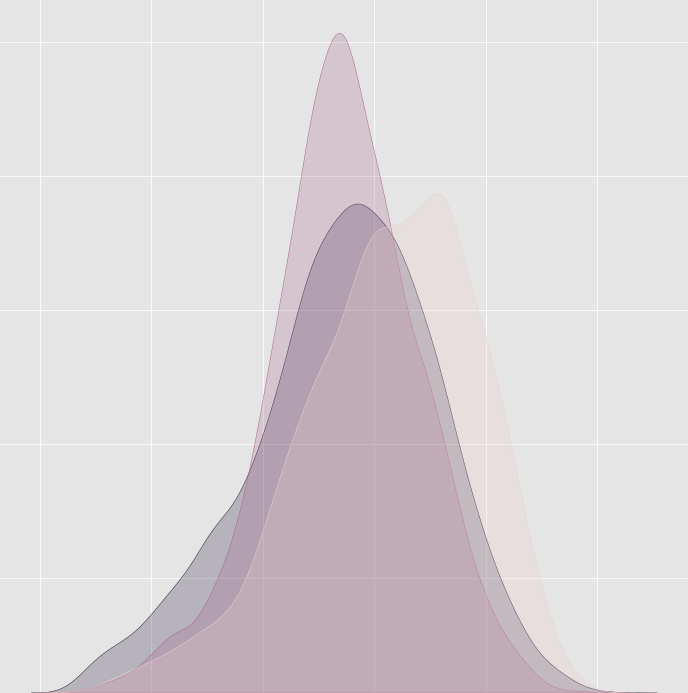
\includegraphics[width=0.35\linewidth]{img/seconds-since-50-trades-ago-BUY.png}
    }
\subfloat[open-close-diff-SELL-30-sec]{
    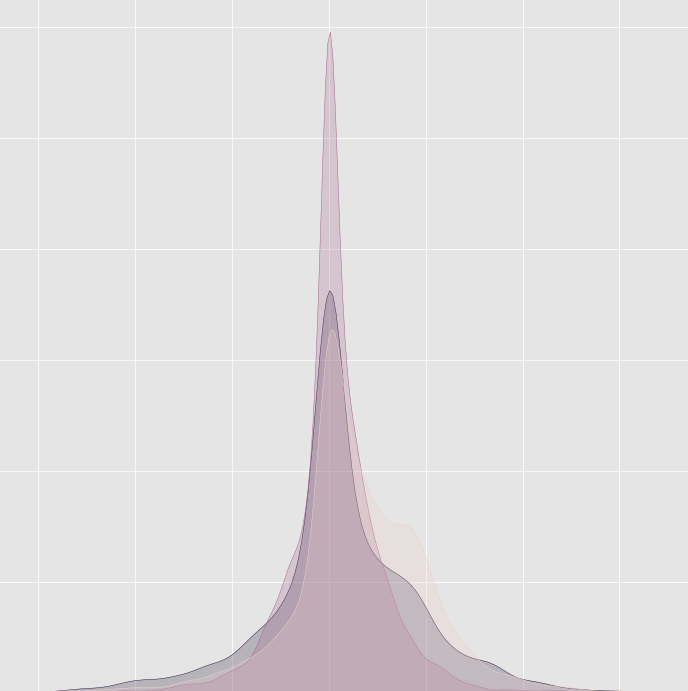
\includegraphics[width=0.35\linewidth]{img/open-close-diff-SELL-30-sec.png}
    }
\end{figure}

Видим, что оба распределения такие, что почти невозможно отличить один таргет от другого, только на \href{fig:trades_ago} можно немного отличить таргет $-1$, который бежевого цвета. Поэтому ждать, что модель у нас получится хорошая не приходится.



\subsection{Результат}
При таких параметрах получается, что моделька в $9.78\%$ случаев с вероятностью $69.63\%$ правильно предсказывает скачок рынка. То есть из всех скачков она ловит только $9.78\%$. И среди них с вероятностью $69.63\%$ угадывает, куда пойдет рынок.

Однако если учитывать комиссию биржи, то мы будем играть в минус.


\section{Арбитражная стратегия}

В нашем проекте мы, конечно, не могли не попробовать одну из самых распространённых и классических стратегий высоко частотного трейдинга -- арбитраж. Идейно в этой стратегии все просто: мы смотрим на цену на одной бирже (сигнальной) и если она резко пошла вверх или вниз, то предпринимаем соответствующие действия на нашей бирже.

\subsection{Описание стратегии}
Если мы засекли быстрое и сильное изменение цены на сигнальной бирже, то выставляем рыночный ордер на нашей бирже в направлении изменения цены. Следом отправляем два ордера, которые будут фиксировать прибыль и убыток. Таким образом, если мы угадали с направлением движения цены, то у нас появляется шанс заработать. Ключевые параметры стратегии:
\begin{itemize}
\item \texttt{Profit threshold} -- от этого параметра зависит, насколько далеко от цены исполнения рыночного ордера мы будем выставлять ордер для фиксации прибыли.
\item \texttt{Loss threshold} -- аналогично предыдущему, но для фиксации убтков.
\item \texttt{Signal threshold} -- показывает, какое изменение в цене мы считаем "сильным",,если на сигнальной бирже оно было больше этого параметра, то можем фиксировать сигнал
\item \texttt{Window size} -- промежуток времени, за который мы фиксируем скачок. Если цена выросла на нужный \texttt{Signal threshold} за \texttt{Window size}, то тогда фиксируем сигнал, если цена росла дольше, чем \texttt{Window size}, то мы не считаем это за сигнал.
\item \texttt{Sec to wait} -- сколько мы держим рыночный ордер. Если по фиксирующим ордерам не прошла сделка и через \texttt{Sec to wait} секунд мы не зафиксировали ни прибыль, ни убыток, то закрываем нашу позицию новым рыночным ордером. 
\end{itemize}




\subsection{Выбор биржи и инструмента}
В мире сейчас очень много криптовалютных бирж, но самой крупной уже долгие годы остается Binance, поэтому мы решили наблюдать за ценой на ней, ведь там совершаются десятки сделок в секунду. Инструментов тоже существует бесчисленное множество, мы остановились на бессрочном фьючерсе биткоина, который торгуется в долларах. Такой выбор был продиктован следующими причинами: биткоин до сих пор остается самой популярной криптовалютой, цена на сам биткоин очень волатильна, а на его фьючерс и подавно, это дает нам возможность ловить большие скачки цены, на бирже dydx в основном представлены бессрочные фьючерсы и нам показалось логичным соверш�ть сделки на основании информации о похожем инструменте.  


\subsection{Обнаружение скачков с помощью скользящего окна}
Одна из ключевых задач в арбитражной стратегии -- обнаружение быстрого и сильного изменения цены. Мы считаем, что цена изменилась быстро, если изменения произошли менее, чем за одну секунду (значит, Window size = 1000 миллисекунд) и сильно, если скачок цены был больше, чем на две комиссии на Binance (значит, Signal threshold = 1 + 2 * Binance Commission + eps). Чтобы обнаруживать такие события, был создан класс SlidingWindow ~\cite{SlidingWindowClass}, реализующий алгоритм поиска минимума в скользящем окне ~\cite{SlidingWindowAlgorithm}, адаптированного под наши нужды. Работает это примерно следующим образом:
\begin{itemize}
\item Мы создаем экземпляр класса SlidingWindow, с указанием размера окна в миллисекундах
\begin{verbatim}
slide = SlidinWindow(window_size)
\end{verbatim}

\item При поступлении нового трейда от вебсокета Binance/при анализе исторических данных, мы парсим данные и обновляем окно, добавляя туда новую цену и timestamp свежего трейда, метод push\_back возвращает True, если минимум или максимум был изменен и False иначе:
\begin{verbatim}
result = slide.push_back(price, timestamp)
\end{verbatim}

\item Далее мы смотрим, если отношение минимума цены к максимуму больше или равно нашего порога, то тогда считаем, что мы поймали скачок, который дальше можно как-то анализировать:
\begin{verbatim}
if result:
    max_in_window = self.slide.get_max()
    max_timestamp = self.slide.get_max_timestamp()
    min_in_window = self.slide.get_min()
    min_timestamp = self.slide.get_min_timestamp()
    if max_in_window / min_in_window >= (
        1 + self.signal_threshold):
            if max_timestamp > min_timestamp:
                return "BUY"
            elif max_timestamp < min_timestamp:
                return "SELL"
\end{verbatim}
\end{itemize}

Этот класс будет использоваться для поиска скачков на исторических данных и для их обнаружения в реальном времени в рабочем прототипе трейдера

\subsection{Анализ исторических данных, реагируем на все сигналы}
Чтобы понять, возможно ли вообще заработать, используя эту стратегию, был проведен анализ исторических данных. Данные с Binance мы брали из публичного архива ~\cite{BinanceArchive}, а данные с dydx собирали простеньким скриптом ~\cite{DyDxCollectData}, впрочем, и в коннекторе есть для этого отдельная функция ~\cite{DyDxCollectDataConnector}.

\subsubsection{Class ProfitCalcualtor}
Для анализа исторических данных и подсчета прибыли был создан класс с говорящим названием \texttt{ProfitCalculator}, который позволяет нам понять, сколько мы теоретически можем заработать, используя арбитражную стратегию. При создании экземпляра этого класса ему обязательно передаются имена файлов, которые содержат исторические трейды с сигнальной биржи и трейды биржи, с которой мы торгуем. Можно также установить ключевые параметры стратегии, но они есть по умолчанию. Выглядит это так:
\begin{verbatim}
PC = ProfitCalcualtor(signal_filename, predict_filename, **params)
\end{verbatim}

\subsubsection{Сбор сигналов}
У класса \texttt{ProfitCalculator} есть метод \texttt{get\_signals}, который позволяет нам получить сигналы на основе трейдов, которые лежали в файле с именем \texttt{signal\_filename}. Мы можем сдампить сигналы, воспользовавшись соответствующими методами класса. И, конечно, визуализировать их тоже можно. То есть стандартный сценарий использования \texttt{ProfitCalculator} с целью получения сигналов такой:
\begin{verbatim}
PC.get_signals()
PC.dump_signals(signals_filename)
PC.show_signals()
\end{verbatim}

Вот пример работы метода \texttt{show\_signals}:
\begin{figure}[H]
\center{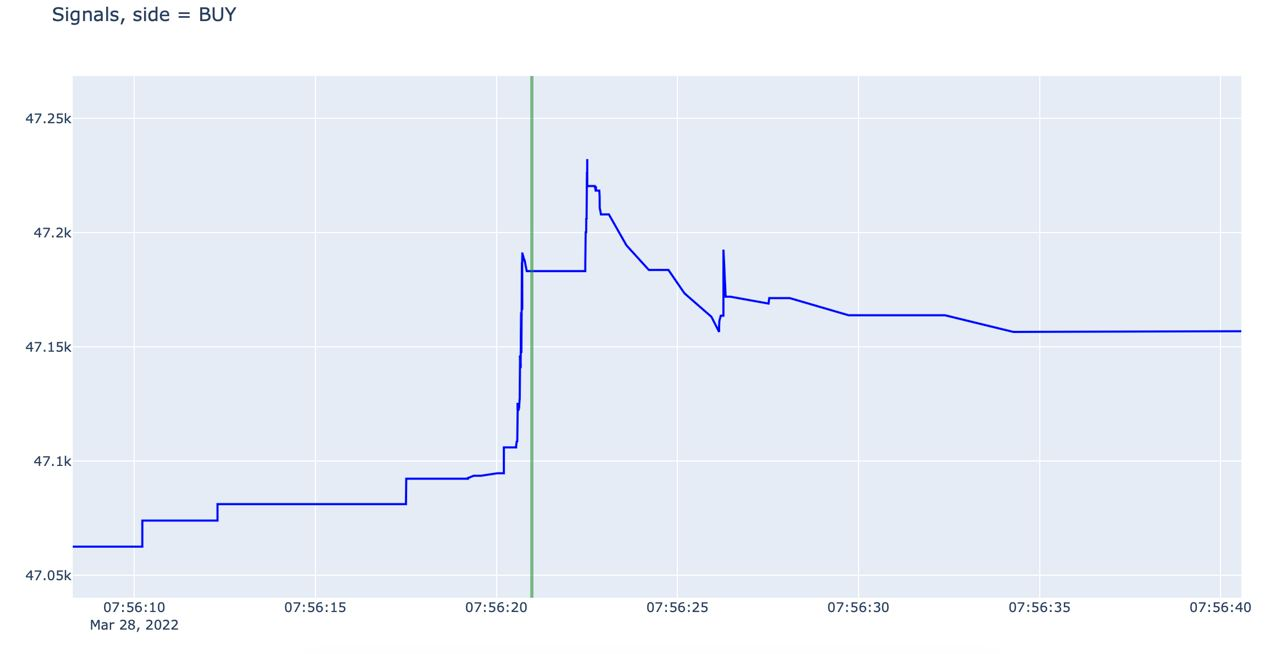
\includegraphics[scale=0.4]{imgs/signal.jpg}}
\caption{BUY signal example}
\label{fig:image}
\end{figure}

\subsubsection{Получение трейдов и расчет прибыли}
После того как мы получили сигналы, можно воспользоваться методам \texttt{get\_trades}, который, имитируя торговлю по арбитражной стратегии на исторических данных из файла  \texttt{predict\_filename}, сохраняет трейды. Далее можно сдампить трейды в файл с помощью метода \texttt{dump\_trades} и получить график, на котором отмечены наши сделки  помощью \texttt{show\_trades}. 
\begin{figure}[H]
\center{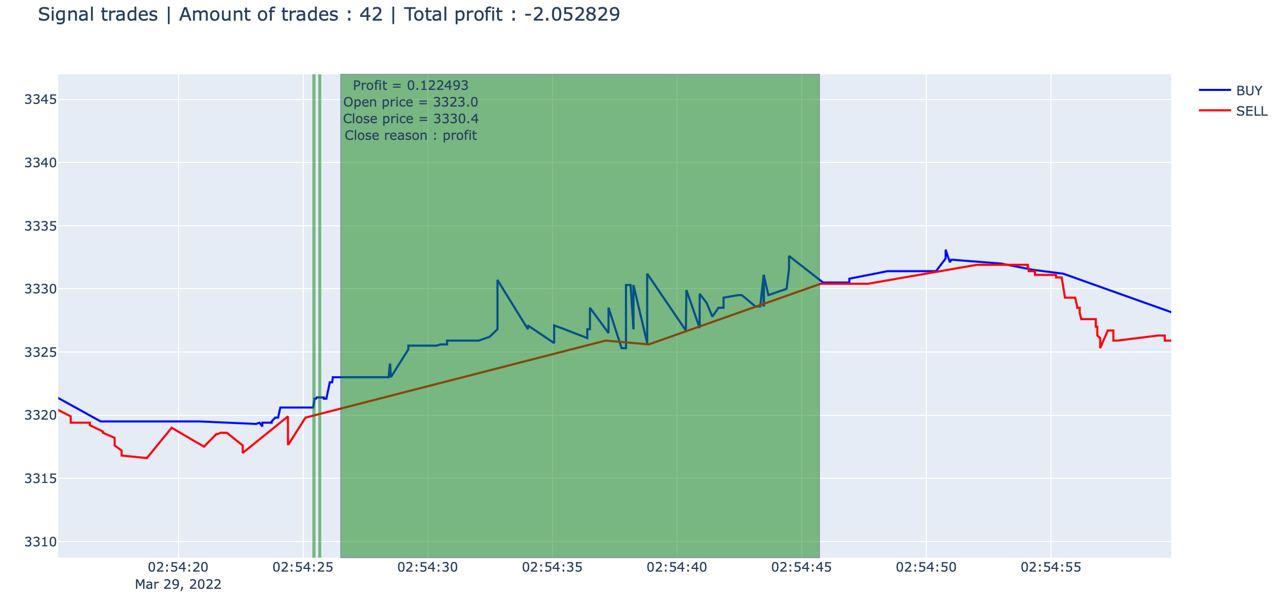
\includegraphics[scale=0.4]{imgs/trade.jpg}}
\caption{BUY trade example}
\label{fig:image}
\end{figure}


Теперь, когда у нас есть трейды, мы можем посчитать, на сколько процентов увеличится наш портфель. Делается это с помощью метода \texttt{get\_profit}, который возвращает нам общий профит со всех циклов открытия и закрытия позиций и список профитов для каждого из них по отдельности. Вот таблица суммарных профитов за несколько месяцев:

\begin{table}[h]
    \centering
    \begin{tabular}[t]{ | l | l | l | l | }
    \hline
    Dec & Jan & Feb & Mar \\ \hline
    5.21 & 6.45 & -6.27 & -17.03 \\
    \hline
    \end{tabular}
    \label{table:satellites}
\end{table}

Эти значения были получены при фиксированных ключевых параметрах на весь месяц. Понятно, что можно с ними немного поиграться с целью увеличения профита, но это не дает больших результатов. Сколько бы мы не экспериментировали с ними, картина остается примерно такой же: в декабре/январе мы что-то зарабатываем, а дальше все очень плохо.







\subsection{Анализ исторических данных, попытка отсеять плохие сигналы}
Как видно из таблицы выше, ситуация скорее печальная, чем радостная. Есть несколько аномальных месяцев, которые принесли бы нам прибыль, но большинство из них все-таки были убыточными. Мы теряем много денег, когда реагируем на плохие сигналы и зарабатываем недостаточно, когда реагируем на хорошие, но выставляем плохие трешхолды. Есть два очевидных пути улучшения нашей стратегии: научиться не реагировать на плохие сигналы, либо уметь подбирать ключевые параметры стратегии для каждого сигнала по отдельности. Поговорим здесь о первом варианте (спойлер: даже он не работает).

\subsubsection{Сбор фичей}
Нам нужно выделить какие-то фичи, по которым мы будем предсказывать, будет ли сигнал прибыльным или нет. Их должно быть удобно собирать, они должны отражать фундаментальные характеристики нашего скачка. Мы выделили следующие признаки:

\begin{itemize}
\item \texttt{Average quantity} -- средняя цена объема сделки в окне.
\item \texttt{Max quantity} -- максимальная цена объема сделки в окне.
\item \texttt{Stdev price} -- стандартное отклонение цены в окне.
\item \texttt{Stdev quantity} -- стандартное отклонение объема в окне.
\item \texttt{Trades frequency} -- частота трейдов в окне.
\item \texttt{Jump value} -- величина прыжка: во сколько раз изменилась цена.
\item \texttt{Jump time length} -- длина прыжка: сколько миллисекунд потребовалось, чтобы достичь \texttt{Jump value}.
\end{itemize}

Все эти признаки легко собирать с помощью стандартного питоновского пакета \texttt{statistics}, добавив еще одно скользящее окно, отслеживающее объем трейдов, вместо их цены. Теперь метод \texttt{get\_signals} будет не только находить сигналы, но и собирать фичи к каждому из них.

\subsubsection{Узнаем, был ли сигнал теоретически прибыльным}
Для этого мы будем идти на 20 секунд вперед от времени сделки по рыночному ордеру, который мы отправили после получения сигнала, и если отношение цены хотя бы одного из трейдов за эти 20 секунд к цене рыночного была \texttt{> 1 + dydx\_commission}, то это значит, что мы могли заработать, отреагировав на этот сигнал. 

Еще по дороге будем собирать наилучшие ключевые параметры стратегии для данного сигнала: какой максимальный \texttt{Profit threshold} мы могли выставить, чтобы заработать как можно больше, какой должен был быть \texttt{Profit threshold}, чтобы не закрыться по нему, зафиксировав прибыль и т.п. Делается это просто, надо всего лишь найти минимальную/максимальную цену на окне в 20 секунд, которые мы анализируем и посчитать отношение цен.

\subsubsection{Пытаемся отличить плохие сигналы от хороших}
        Теперь у нас есть матрица вида

\begin{table}[h]
    \centering
    \begin{tabular}[t]{ | l | l | l | l | }
    \hline
    Average quantity & Max quantity & ... & Has profit \\ \hline
    100 & 1000 & ... & 1 \\
    ... & ... & ... & 0 \\
    ... & ... & ... & ... \\
    \hline
    \end{tabular}
    \label{table:satellites}
\end{table}

И мы можем попробовать поприменять к этим данным различные модели классификации, чтобы научиться отличать успешные сигналы. Но для начала посмотрим на совместное распределение фичей. Может удастся увидеть какую-то структуру в данных. 

\begin{figure}[H]
\center{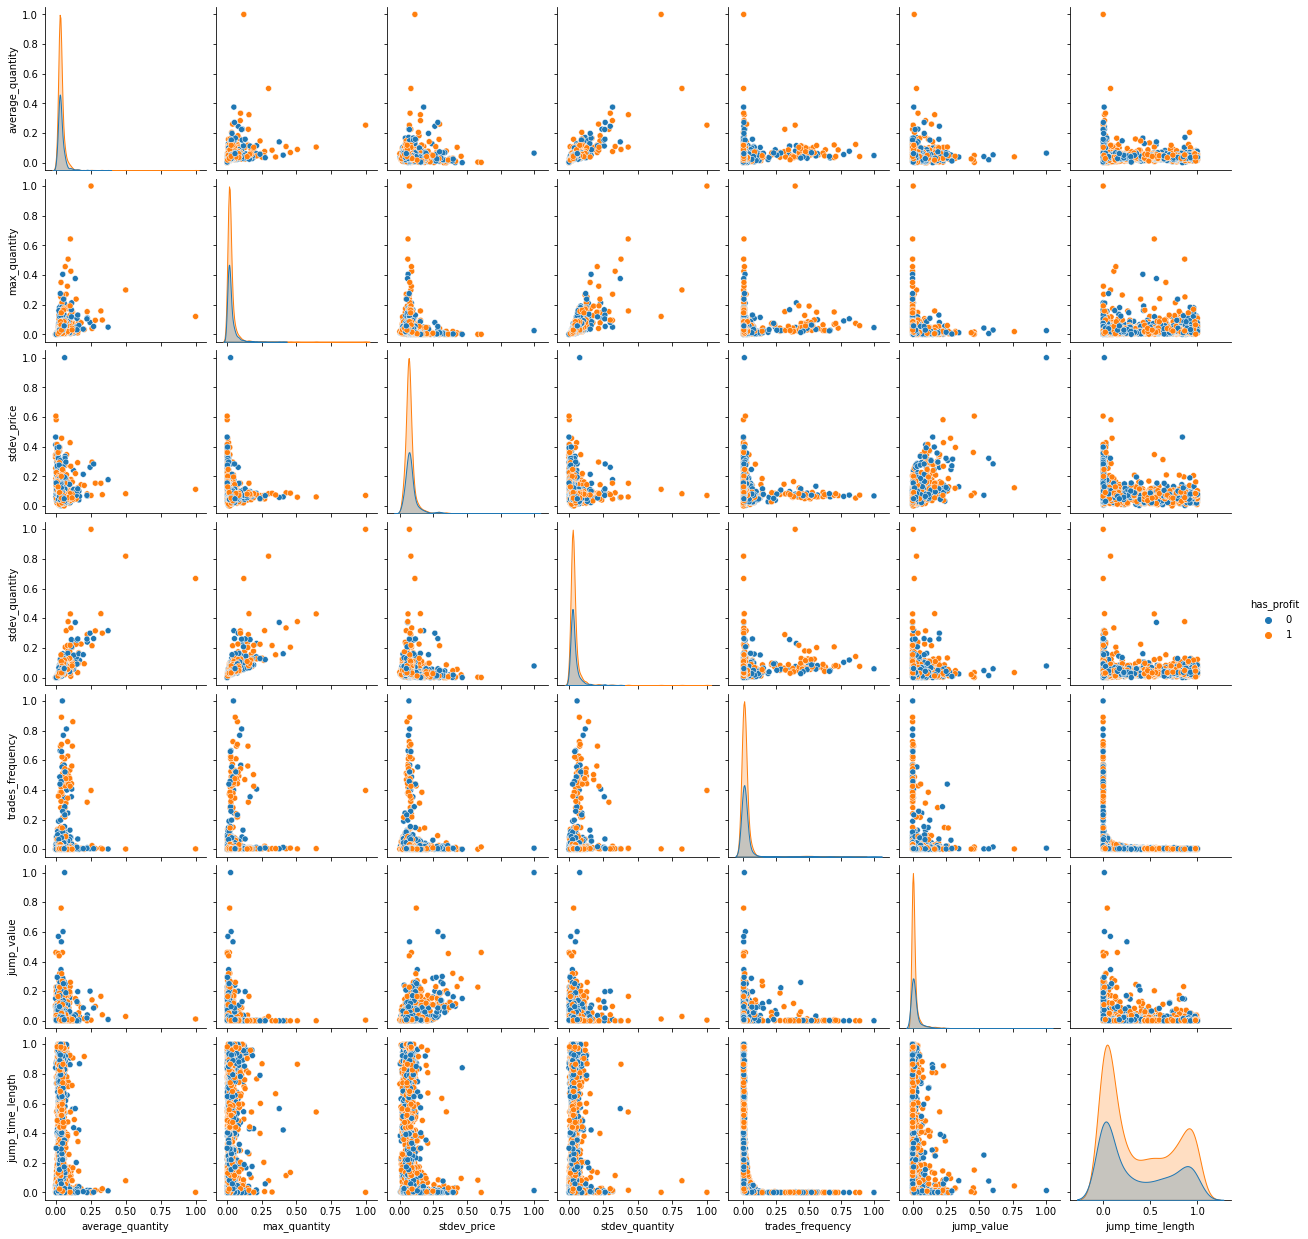
\includegraphics[scale=0.4]{imgs/features.png}}
\caption{Feature's distribution}
\label{fig:image}
\end{figure}

Видно, что классы очень плохо отделяются, все перемешано, шансов на хорошую классификацию очень мало. Но мы попробуем (но ничего не получиться).

\begin{itemize}
\item \textbf{Решающие деревья}

Пользуемся \texttt{DecisionTreeClassifier} из \texttt{sklearn}. Для хорошей интерпретируемости ограничим глубину дерева одним уровнем. Это даст нам понимание, какой самый значимый признак выделил классификатор.
\begin{verbatim}
from sklearn.tree import DecisionTreeClassifier
model = DecisionTreeClassifier(max_depth=1)
model.fit(X_train, Y_train_has_profit)
model.score(X_test, Y_test_has_profit)
\end{verbatim}

Результаты не очень хорошие: средняя точность составляет всего 69\%. Посмотрим на визуализацию нашего небольшого дерева:
\begin{figure}[H]
\center{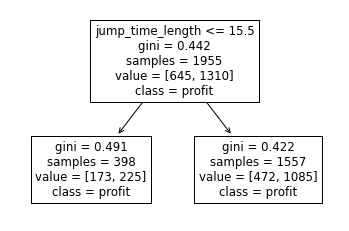
\includegraphics[]{imgs/tree1.png}}
\caption{Decision Tree}
\label{fig:image}
\end{figure}

Видно, что gini-коэффициент в каждой вершине довольно близок к 0.5, это означает, что данный признак плохо разделяет классы. В каждой вершине находится много сигналов обоих типов. Общее число успешных сигналов во всем нашем датасете составляет где-то 66\%. Если мы будем игнорировать все сигналы,  \texttt{Jump time length} которых меньше 100мс, то можем повысить долю успешных сигналов до 68\%:

\begin{verbatim}
>>> print(f"Было: {df_total[df_total.has_profit == 1].shape[0] 
                                                / df_total.shape[0]}")
Было: 0.6617752326413744
>>> df_total = df_total[df_total.jump_time_length > 100]
>>> print(f"Стало: {df_total[df_total.has_profit == 1].shape[0] 
                                                / df_total.shape[0]}")
Стало: 0.6815804764671702
\end{verbatim}

Можно еще раз повторить процедуру с DecisionTreeClassifier, но уже с отфильтрованным датасетом, получим такую картинку:
\begin{figure}[H]
\center{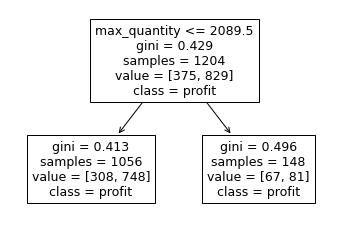
\includegraphics[]{imgs/tree2.png}}
\caption{Decision Tree}
\label{fig:image}
\end{figure}

Ну тоже, мягко говоря, не очень получается, но давайте опять отфильтруем датасет по этому признаку и посмотрим, возросла ли доля хороших сигналов:
\begin{verbatim}
>>> print(f"Было: {df_total[df_total.has_profit == 1].shape[0] 
                                                / df_total.shape[0]}")
Было: 0.6815804764671702
>>> df_total = df_total[df_total.max_quantity <= 2100]
>>> print(f"Стало: {df_total[df_total.has_profit == 1].shape[0] 
                                                / df_total.shape[0]}")
Стало: 0.6950732356857523
\end{verbatim}

Ну опять как-то не радостно. Можем теперь посчитать профит на разных месяцах, отсекая сигналы, у которых \texttt{Jump time length} < 100 и \texttt{Max quantity} > 2100. Получим следующие профиты:

\begin{table}[h]
    \centering
    \begin{tabular}[t]{ | l | l | l | l | }
    \hline
    Dec & Jan & Feb & Mar \\ \hline
    5.21 & 6.45 & -6.27 & -17.03 \\
    \hline
    \end{tabular}
    \label{table:satellites}
\end{table}

Ситуация практически не изменилась, а мы ведь так старались! 

\item \textbf{Другие модели}

Мы также попробовали другие модели бинарной классификации: логистическая регрессия, решающие деревья с градиентным бустингом, даже какие-то совсем базовые нейросети. Но ничего не дает внушительного результата, который бы позволял нам зарабатывть больше.
\end{itemize}

Что касается попытки предсказывать ключевые параметры стратегии, то она была обречена на провал, ведь если задуматься, одной из характеристик модели, которая бы предсказывала параметры, как раз является умение отличить плохой сигнал от хорошего, а мы это сами не смогли сделать. Попробовали разные виды линейных регрессий с регуляризацией, различные регрессоры, основанные на решающих деревьях, но все это не принесло никаких хороших результатов. Очень жаль! �


\section{Трейдер}

\href{https://github.com/dexety/dex-trading-system/blob/main/strategy/arbitrage/trader.py}{Трейдер в репозитории}

\begin{definition}
\textbf{Трейдер} -- программа, которая на основе готовой стратегии, совершает сделки.
\end{definition}

\subsection{Использованные технологии}

\subsubsection{\texttt{Асинхронная функция}}

\begin{definition}
\textbf{Асинхронная функция} -- функция, которая не блокирует основой поток программы.
\end{definition}

Наш проект написан на питоне, а он одно-поточный. Поэтому нужно было пользоваться всеми возможностями асинхронности. Для этого в питоне есть очень простой интерфейс:

\begin{verbatim}
async def slow_calculation():
    return ...
    
async def hard_calculation():
    return ...
    
def main():
    loop = asyncio.get_event_loop()
    loop.create_task(
        slow_calculation(), name="slow_calculation"
    )
    loop.create_task(
        hard_calculation(), name="hard_calculation"
    )
    loop.run_forever()
\end{verbatim}

Здесь мы создали две задачи: \texttt{slow\_calculation} и  \texttt{hard\_calculation}, которые будут выполняться асинхронно, то есть не мешать друг другу своим вычислениями.

\subsubsection{\texttt{asyncio.Event}}

В трейдере, помимо асинхронных функций, используется класс \texttt{asyncio.Event}, позволяющий ждать задачам, пока событие не произойдет в другой задаче и элемент класса не будет разблокирован.

\begin{verbatim}
async def waiter(event):
    print('waiting for it ...')
    await event.wait()
    print('... got it!')

async def main():
    # Create an Event object.
    event = asyncio.Event()

    # Spawn a Task to wait until 'event' is set.
    waiter_task = asyncio.create_task(waiter(event))

    # Sleep for 1 second and set the event.
    await asyncio.sleep(1)
    event.set()

    # Wait until the waiter task is finished.
    await waiter_task

asyncio.run(main())
\end{verbatim}

В данном примере функция \texttt{waiter} не завершится до тех пор, пока функция \texttt{main} не разблокирует событие строчкой \texttt{event.set()}, потому что \texttt{waiter} находится в ожидании после строчки \texttt{await event.wait()}.

С помощью этого класса можно синхронизировать работу алгоритма торговли с ответами от биржи.

\subsection{Устройство трейдера}

Используемые параметры:
\begin{itemize}
    \item \href{https://github.com/dexety/dex-trading-system/blob/ca0370d602f2dfa05262b9b8574002f965ac1502/research/ib-0002-cross-analysis/trader.py#L52}{\texttt{trailing\_percent}} -- процент, на который цена stop-loss ордера отстает от рыночной при отправке trailing-stop ордера.
    \item \href{https://github.com/dexety/dex-trading-system/blob/ca0370d602f2dfa05262b9b8574002f965ac1502/research/ib-0002-cross-analysis/trader.py#L54}{\texttt{profit\_threshold}} -- процент, на который цена лимитки, выставленной по take-profit ордеру отличается от рыночной.
    \item \href{https://github.com/dexety/dex-trading-system/blob/ca0370d602f2dfa05262b9b8574002f965ac1502/research/ib-0002-cross-analysis/trader.py#L55}{\texttt{sec\_to\_wait}} -- количество секунд, через которое цикл торговли считается завершенным, если ни take-profit, ни trailing-stop ордеры не были исполнены.
\end{itemize}

Трейдер состоит из двух асинхронных задач и вспомогательных функций. 

Из ключевых вспомогательных функций нужно отметить функцию \href{https://github.com/dexety/dex-trading-system/blob/main/research/ib-0002-cross-analysis/trader.py#L303}{\texttt{reset}}, которая переводит все поля класса в состояние для ожидания скачка на бинансе. Она вызывается после успешного завершения цикла торговли, или после отмены ордеров и закрытия позиции в случае, когда какой либо ордер не смог исполниться.

Основные асинхронные задачи:
\begin{itemize}
    \item \texttt{listen\_binance}
    \item \texttt{account\_listener}
\end{itemize}

Пройдемся по каждой

\subsubsection{\texttt{listen\_binance}}

\href{https://github.com/dexety/dex-trading-system/blob/main/research/ib-0002-cross-analysis/trader.py#L167}{Функция в репозитории}

\begin{definition}
\textbf{Слушать [что-то]} -- значит подключиться по веб-сокету к какому-то серверу и получать от него обновления.
\end{definition} 

Эта функция реализует логику торговли. В этом трейдере по техническим причинам не получилось использовать функционал коннектора для бинанса, поэтому подписываться на обновления пришлось в ручную. Функция держит окно трейдов на одном направлении фиксированной длины, и если перепад цены превысил порог, то запускается алгоритм торговли:

\begin{enumerate}
    \item Отправляется маркет ордер. Функция входит в режим ожидания с помощью \texttt{asyncio.Event} и ждет, пока с биржи придет ответ об исполнении ордера. Если с биржи приходит сообщение об отмене ордера, то вызывается функция \texttt{reset} и трэйдер возвращается в состояние ожидания скачка цены на бинансе.
    \item Когда \texttt{account\_listener} сообщил об успешном выполнении маркет ордера и сохранил цену по которой он исполнился, трейдер выставляет \texttt{take-profit} и \texttt{trailing-stop} ордеры с заданными при инициализации класса параметрами и на протяжении \texttt{sec\_to\_wait} секунд ожидает исполнения хотя бы одного из них.
    \begin{itemize}
        \item Если за \texttt{sec\_to\_wait} секунд ордеры не закрылись, то они отменяются. Далее закрывается позиция в которую мы зашли маркетом, и когда с биржи приходит сообщение о закрытии позиции, цикл торговли считается завершенным.
        \item Если какой-то из ордеров исполнился, то мы в любом случае отменяем оставшийся. Если исполнился лимит, то мы в плюсе, если трэйлинг стоп, то, скорее всего, в минусе. После отмены цикл считается завершенным.
    \end{itemize}
    
\end{enumerate}


\subsubsection{\texttt{account\_listener}}

\href{https://github.com/dexety/dex-trading-system/blob/main/research/ib-0002-cross-analysis/trader.py#L365}{Функция в репозитории}

Эта задача слушает изменения в наших ордерах и позициях, обновляет цену, по которой исполнился маркет, выставляет флаги и разблокирует нужные события, на которых спит функция \texttt{listen\_binance}, тем самым обеспечивая её синзронизацию с биржей.


\section{Заключение}
\subsection{Результаты}
\subsubsection{Коннекторы}
Для взаимодействия с биржей был написан класс, использующий API. Класс предоставляет множество различных методов для алгоритмического трейдинга и может быть использован во многих проектах похожей направленности.
\subsubsection{Market Making}
Попробовали реализовать стратегию market making'a, которая не очень хорошо сработала в наших реалиях, но может быть успешной в рамках децентрализованной торговли, если снизятся комиссии в ETH-2 (очень этого ждем).
\subsubsection{Торговля на основе индикаторов}
Была написана стратегия торговли, базирующаяся на информации об индикаторах. На основе информации о них с помощью библиотеки катбуст мы попытались предсказывать направление движения рынка. Наша стратегия не очень сработала, так как классы были трудно различимы.
\subsubsection{Арбитраж}
Предприняли попытку реализовать стратегию, которая торгует исходя из курса на другой бирже. Для этого написали инструмент, позволяющий рассчитать теоретическую прибыль. Попробовали отделять теоретически прибыльные сигналы от убыточных. 

Написали трейдера для этой стратегии, он слушает вебсокет Binance и торгует на dydx. Вот что-что, а трейдер получился не плохим, очень идиоматично написан, использует немного ресурсов и прост в понимании. Вот бы еще и стратегия работала.

\subsection{Дальнейшие перспективы}
\subsubsection{Разработка инфраструктуры для сбора информации}
По ходу написания и тестирования различных стратегий нами было написано множество различных инструментов для сбора и анализа, которые можно развить в полноценную библиотеку для сбора и анализа данных информации с основных бирж.
\subsubsection{Улучшение имеющихся стратегий}
Можно попробовать доделать уже имеющиеся стратегии. Существует очень много вариантов апгрейда наших наработок. Рассмотрим каждую из стратегий.
\begin{itemize}
    \item \textbf{Market Making}
    \item \textbf{Индикаторы}
    
    Можно придумать новые индикаторы, которые будут использоваться при классификации. Можно обратиться к уже имеющимся вариантам и подыскать там что-то подходящее. Рассмотрение других индикаторов, возможно, приведет к лучшему отделению классов друг от друга. 
    
    Также не стоит забывать о большом количестве моделей для классификации, которые можно использовать для поставленных задач. Быть может, какая-то из них даст нам лучший результат.
    
    В нашей реализации мы никак не использовали данные со стакана. Дальнейшее развитие может заключаться именно в этом: как-то анализировать не только совершенные сделки, но и смотреть, как ведут себя все участники рынка.
    \item \textbf{Арбитраж}
    
    В этой стратегии стоит работать в направлении поиска новых фичей, которые могли бы помочь отделить теоретические успешные сигналы от провальных. Также можно посмотреть в сторону разработки инструмента для подбора ключевых параметров стратегии. Можно слушать несколько бирж и пробовать каким-то образом усреднять сигналы. 
    
    Следует оптимизировать трейдер, возможно, переписать его на другой, более быстрый язык программирования, ведь здесь нам важна каждая миллисекунда.
    
    Попытаться найти географическое положение, в котором задержка до сигнальной биржи и до той, на которой мы торгуем, будет минимальная. В этой стратегии такой характер задержки носит принципиальный характер.

\subsubsection{Поиск новых бирж и инструментов}
Конечно, всегда можно попытаться найти какую-то свежую биржу, на которой еще не расплодились боты всяких HFT фондов, и попробовать уже написанные стратегии. Вполне вероятно, что какое-то время они могут приносить деньги. Главное вовремя понять, когда это закончиться. И следует обратить внимание на другие инструменты и валюты, которые мы обошли стороной. На них успех тоже возможен.

\subsubsection{Переход к по-настоящему децентрализованным технологиям}
Можно направить проект немного в другое русло и рассмотреть торговлю непосредственно в сети эфира. Это уже влечет написание смарт-контрактов и тому подобное. Надо основательно разобраться в блокчейне и изучить технологии. Но тогда нам откроется множество новых подходов к алгоритмическому трейдингу. Они могут быть крайне прибыльными.
    
\end{itemize}


\section{Дополнительный результаты}

Помимо задач, которые нам поставил руководитель, мы сделали еще:

\subsection{Визуализация}
Перед тем, как работать с данными, надо понять, как они устроены: попарное распределение классов, плотность каждого из индикаторов. Мы все это сделали. Теперь стало гораздо проще подбирать параметры для модели машинного обучения.

\subsection{Маркет-Мэйкинг стратегия}
Это стратегия, когда мы держим окно из зеркальных заявок на каком-то уровне от индекс-цены. Утверждается, что если нас пробили с одной стороны, то почти сразу пробьют и со второй стороны, и мы окажемся в плюсе. Но все оказалось не так: при пробитии нас с одной стороны, рынок продолжал идти в ту же сторону.

\subsection{Контролирующий бот}
Мы сделали телеграм бота, на которого можно по паролю подписаться и получать обновления состояния аккаунта на бирже. Это полезно, когда ты запускаешь торговую стратегию, куда-то отходишь, но при этом всегда можешь контролировать, что с ней происходит, через телеграм.

\subsection{CI/CD, тесты, линтер}
Любая ошибка в торговой системе может потерять наши деньги, поэтому важно, чтобы весь код всегда был рабочим. Для этого мы все, что смогли, обложили тестами c использованием утилиты PyTest~\cite{Pytest}. Теперь при каждом пулл реквесте у нас запускается тестирующая система, и если какие-то тесты не проходят, то мы запрещаем дальнейший пуш. Реализовали мы это через GitHub Actions~\cite{GitHubActions}.

Еще нам хочется, чтобы весь код был консистеным. Для этого мы используем линтер Black~\cite{Black} и статический анализатор PyLint~\cite{Pylint}. В совокупности эти утилиты поддерживают консистентность нашего кода и могут еще до запуска теста, выдать синтаксические ошибки.

\subsection{Смарт контракты}
С помощью смарт контрактов можно занимать у других людей миллиарды, трейдить на них, и потом возвращать криптовалюту обратно. Звучит заманчиво. Мы написали смарт конракты на Solidity~\cite{Solidity}, и залили их в сеть эфира через Brownie~\cite{Brownie}.


% Здесь автоматически генерируется библиография. Первая команда задает стиль оформления библиографии, а вторая указывает на имя файла с расширением bib, в котором находится информация об источниках.
\bibliographystyle{plainurl}
\bibliography{bibl}

% Здесь текст документа заканчивается
\end{document}
% Начиная с этого момента весь текст LaTeX игнорирует, можете вставлять любую абракадабру.
